
%============================================================
\subsection{\texttt{prism}}
\label{subsec:geometry_prism}
%============================================================

\noindent
\textbf{Geometry ID:} \texttt{GLOB-GEO0001}
\qquad
\textbf{Version:} \texttt{1.0.0}

\begin{figure}[htbp]
    \centering
    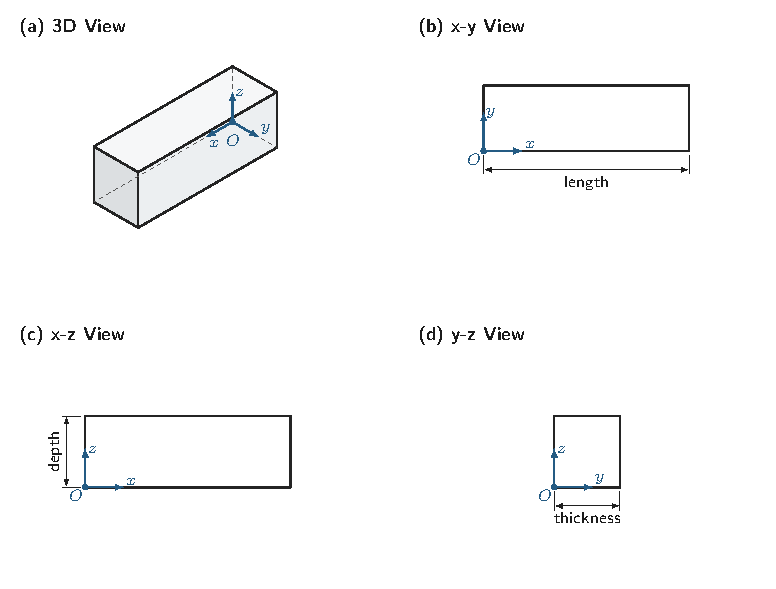
\includegraphics[width=0.7\linewidth]
    {./figs/geometries/prism.pdf}
    \caption{Standardized parametrization and local
    coordinate system of the prism geometry.}
    \label{fig:prism}
\end{figure}

The \texttt{prism} geometry represents a rectangular
prismatic specimen. As illustrated in
Fig.~\ref{fig:prism}, the local coordinate system
is defined by the right-handed Cartesian axes
$x$, $y$, and $z$, with the origin located at
the reference corner indicated in the figure.

The $x$ axis represents the longitudinal direction,
the $y$ axis the transverse thickness direction,
and the $z$ axis the specimen depth direction.

\paragraph{Independent parameters.}

The geometry is defined by three required parameters,
all expressed in millimeters:

\begin{itemize}
    \item \texttt{length}: specimen dimension along
    the local $x$ axis;

    \item \texttt{thickness}: specimen dimension
    along the local $y$ axis;

    \item \texttt{depth}: specimen dimension along
    the local $z$ axis.
\end{itemize}

\paragraph{Geometric constraints.}

All three parameters must be strictly positive.

